\documentclass[11pt,english]{article}
\usepackage[T1]{fontenc}
\usepackage[latin9]{inputenc}
\usepackage{geometry}
\geometry{verbose,tmargin=1.5cm,bmargin=1.5cm,lmargin=1.5cm,rmargin=1.5cm}
\setlength{\parskip}{\bigskipamount}
\setlength{\parindent}{0pt}
\usepackage{babel}
\usepackage{color}
\usepackage[capposition=top]{floatrow}
\usepackage{placeins}
\usepackage{subcaption}
\usepackage{array}
\usepackage{multirow}
\usepackage{amsmath}
\usepackage{amssymb}
\usepackage{graphicx}
\usepackage{afterpage}
\usepackage{rotating}
%\usepackage{epstopdf}
\usepackage[outdir=./]{epstopdf} % Specify the output directory for pdf figures that are converted from eps. Without this, latex cannot read eps figures on mac.
%\usepackage{epstopdf}

\usepackage{esint}
\usepackage[authoryear]{natbib}
\usepackage[unicode=true,pdfusetitle,
bookmarks=true,bookmarksnumbered=false,bookmarksopen=false,
breaklinks=false,pdfborder={0 0 1},backref=false,colorlinks=false]
{hyperref}
\hypersetup{
	citecolor=red,urlcolor=red,linkcolor=red}
\setcounter{MaxMatrixCols}{10}

\setcounter{MaxMatrixCols}{10}

\geometry{verbose}
\PassOptionsToPackage{normalem}{ulem}
\hypersetup{
	plainpages=false,urlcolor=magenta,citecolor=magenta,linkcolor=blue,pdfstartview=FitH,pdfview=FitH,plainpages=false,urlcolor=blue,citecolor=blue,linkcolor=blue,pdfstartview=FitH,pdfview=FitH}



\makeatletter

%%%%%%%%%%%%%%%%%%%%%%%%%%%%%% LyX specific LaTeX commands.
%% Because html converters don't know tabularnewline
\providecommand{\tabularnewline}{\\}

%%%%%%%%%%%%%%%%%%%%%%%%%%%%%% User specified LaTeX commands.


\newcommand*{\FigDir}{../figures} % Folder where figures are stored

\def\indep{\perp\!\!\!\perp}


\def\limfunc#1{\mbox{\rm #1}\,}
\def\d{\,\mathrm{d}}

\usepackage{fullpage}
\usepackage{amsfonts}
\usepackage[titletoc]{appendix}
\usepackage[font=small,labelfont=bf]{caption}
\usepackage{booktabs}
\makeatother

\begin{document}

\title{Tax Avoidance Paper: Report V47 Fixed ``pen''}
\maketitle

We report robustness check results. In counterfactual experiments, we set the pension level to be fixed at the benchmark level (so that the pension replacement rate varies). In doing so, the total abount of benefits $B$ is fixed at the benchmark level.
\section{No Avoidance Experiments \label{sec:exp}}

\begin{itemize}
\item Experiment 3: No avoidance on both margins (i.e. no income shifting and all entrepreneurs are taxed as sole-prop.)
\item Experiment 4: No avoidance on both margins, and the policy function for occupational and legal form choice is fixed at the benchmark model.
\item Experiment 5: All entrepreneurs are sole proprietors (same financial frictions and same taxes).
\end{itemize}

We summarize the results of the experiments in Table \ref{tab:exp_summary}. What's new with respect to the draft: we fixed pen and we added experiment 5.

\begin{table}[htbp]
	\centering
	\begin{tabular}{lccc}
		\toprule
		& Exp. 3 & Exp. 4 & Exp. 5\\
		\hline
		\multicolumn{4}{l}{\textit{Impact on prices}} \\
		Interest rate (p.p.) & -0.57 & -0.20 & 0.10 \\
		Wage (\%) & 3.65 & 1.26 & -0.61 \\
		\multicolumn{4}{l}{\textit{Impact on aggregates}} \\
		Aggregate output (\%) & 7.41 & 1.84 & -2.93 \\
		Aggregate capital (\%) & 10.39 & 4.42 & -2.32 \\
		Ave. entrepreneurial capital (\%) & 39.94 & 9.72 & -13.96 \\
		Entre. Share of output (p.p.) & 11.49 & 1.27 & -5.06 \\
		\multicolumn{4}{l}{\textit{Impact on taxes}} \\
		Total revenue (excl. soc. sec., \%) & 6.52 & -1.44 & -9.57 \\
		Social security contributions (\%) & 0.00 & 0.00 & 0.00 \\
		Social security tax rate (p.p.) & -1.30 & -0.77 & -0.60 \\
		\multicolumn{4}{l}{\textit{Impact on entrepreneurial sector}} \\
		Share of entrepreneurs (p.p.) & -0.45 & -0.35 & 0.42 \\
		Sole prop. As share of entre. (p.p.) & -35.55 & -0.72 & 32.52 \\
		S-corp. as share of entre. (p.p.) & -24.18 & -0.34 & -24.18 \\
		C-corp. as share of entre. (p.p.) & 59.72 & 1.05 & -8.34 \\
		\bottomrule	
		\end{tabular}%
	\caption{Summary of experiments}
	\label{tab:exp_summary}%
	\floatfoot{\textit{Notes:} In counterfactual economies in this table, we assume all model and tax parameters as in the benchmark model. We assume that the social security budget is balanced. To highlight the effects of eliminating tax-avoidance opportunities on tax revenue, we do not adjust the income tax parameter $\lambda_i$ to balance the government budget constraint. Assuming fiscal neutrality does not change the qualitative results besides total tax revenue.}

\end{table}%

\begin{figure}[htbp]
	\centering
	\begin{subfigure}[b]{0.46\textwidth}
		\centering
		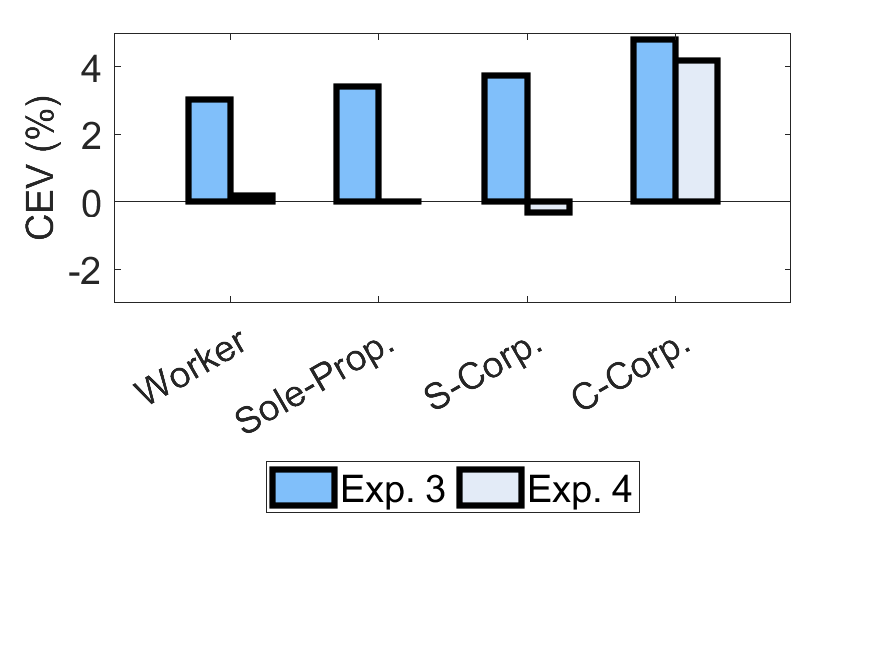
\includegraphics[width=\textwidth]{\FigDir/exp/cev_z_exp3_4}
		\caption{CEV by occupation and LFO}
	\end{subfigure} 
	\begin{subfigure}[b]{0.46\textwidth}
		\centering
		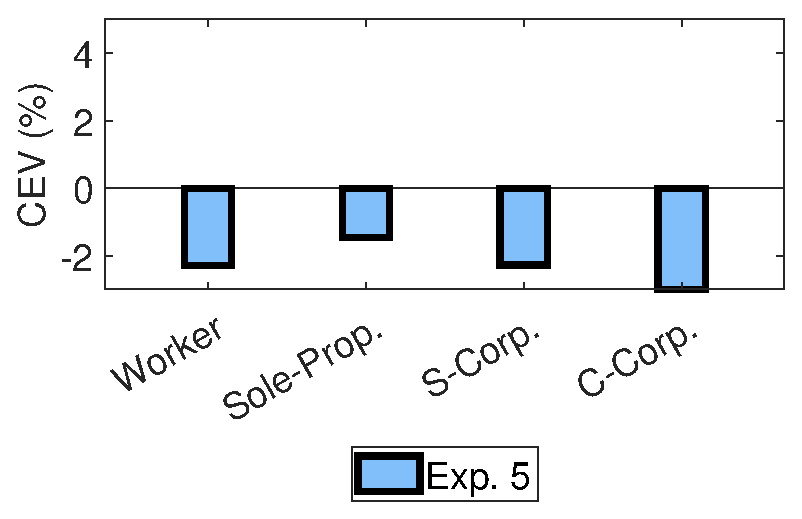
\includegraphics[width=\textwidth]{\FigDir/exp/cev_z_exp5}
		\caption{CEV by occupation and LFO}
	\end{subfigure}
	
	\caption{}
	\label{fig:exp_cev}
	\floatfoot{\textit{Notes:} We assume fiscal neutrality in counterfactual economies and consider transitional dynamics. Each wealth bin contains a quarter of the young population, ordered from the poorest to the richest.}
\end{figure}
\FloatBarrier



\section{Welfare maximization with transition}





%%%
\begin{figure}[htbp]
	\centering
	\begin{subfigure}[b]{0.49\textwidth}
		\centering
		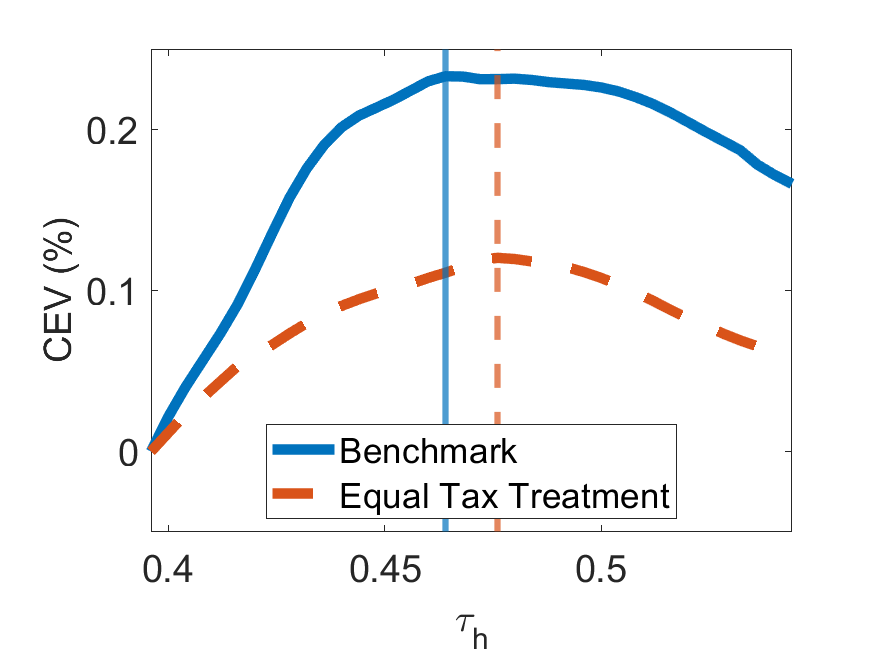
\includegraphics[width=\textwidth]{\FigDir/comptran_cev_vec}
		\caption{Aggregate CEV}
	\end{subfigure}
	\begin{subfigure}[b]{0.49\textwidth}
		\centering
		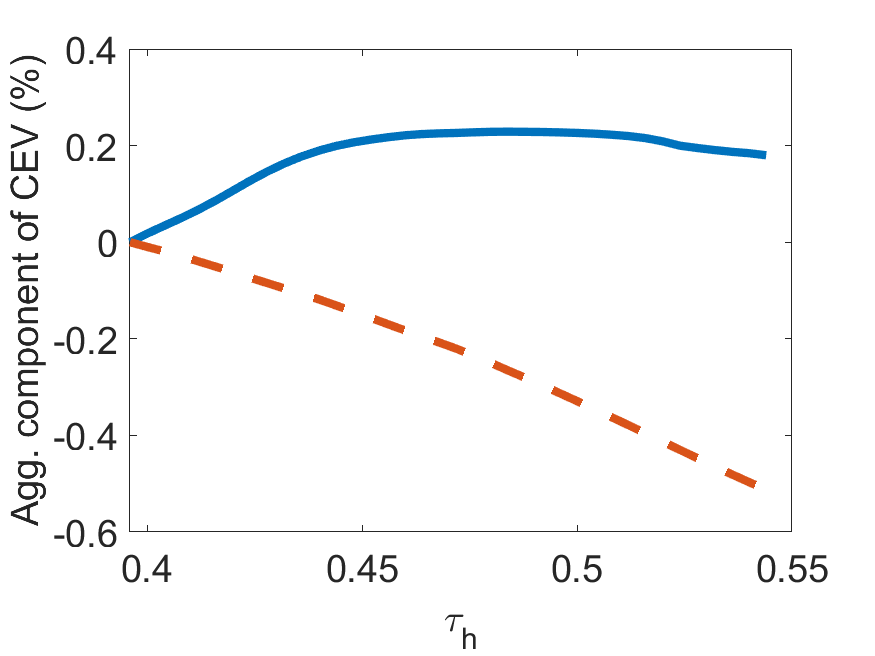
\includegraphics[width=\textwidth]{\FigDir/comptran_cev_aggcomp_vec}
		\caption{Aggregate Component of CEV}
	\end{subfigure} 

	\begin{subfigure}[b]{0.49\textwidth}
		\centering
		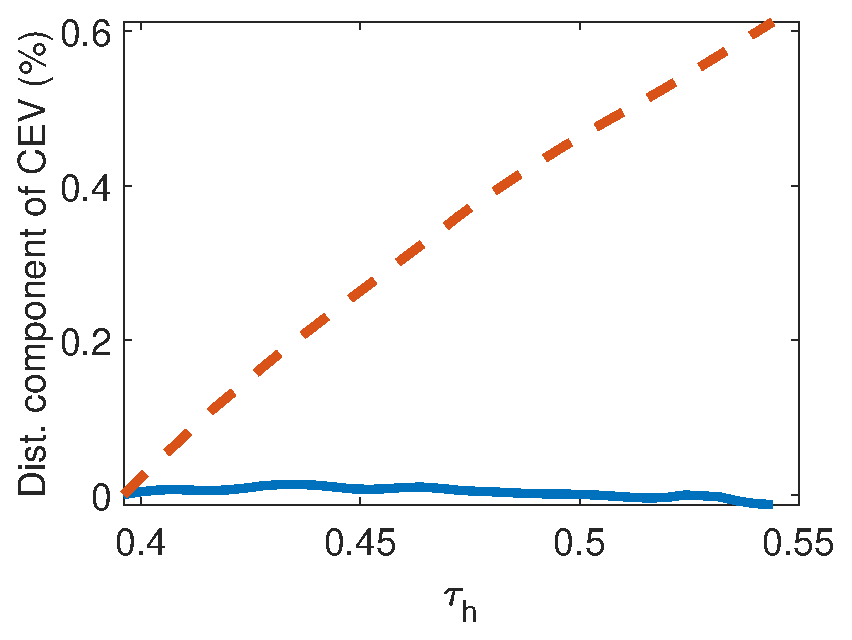
\includegraphics[width=\textwidth]{\FigDir/comptran_cev_distcomp_vec}
		\caption{Distributional Component of CEV}
	\end{subfigure} 
	\begin{subfigure}[b]{0.49\textwidth}
	\centering
	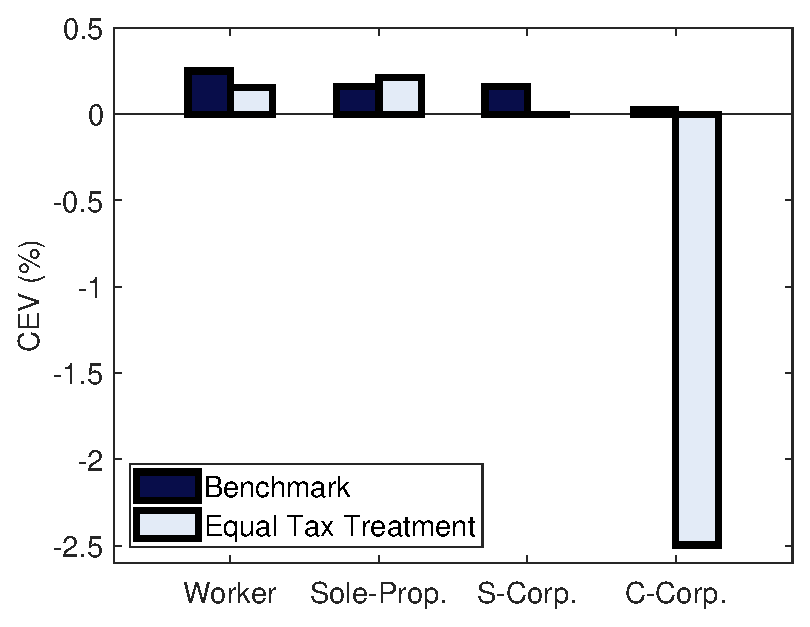
\includegraphics[width=\textwidth]{\FigDir/comptran_cev_z}
	\caption{CEV by occupation and LFO}
\end{subfigure} 

\begin{subfigure}[b]{0.49\textwidth}
	\centering
	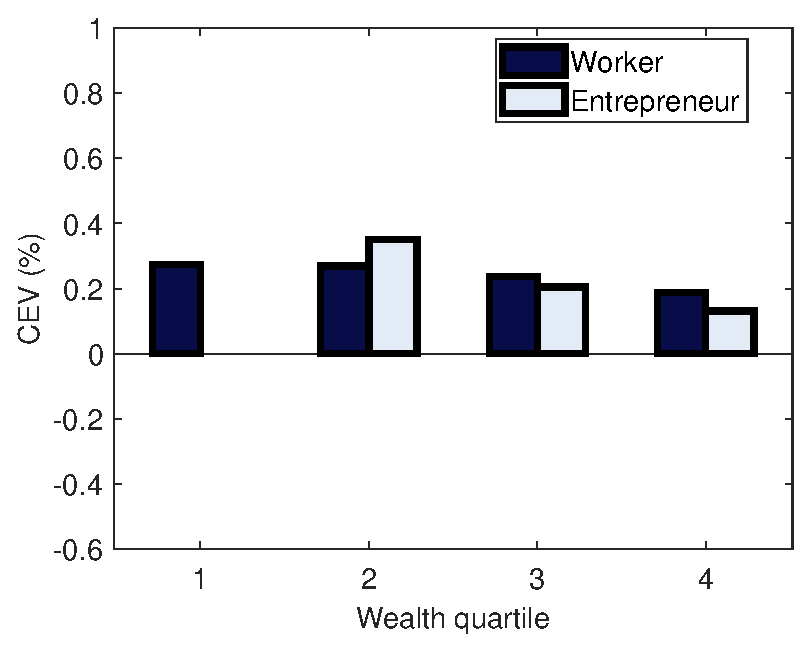
\includegraphics[width=\textwidth]{\FigDir/comptran_base_cev_qo}
	\caption{CEV by wealth decile and occupation, benchmark}
\end{subfigure} 	
\begin{subfigure}[b]{0.49\textwidth}
	\centering
	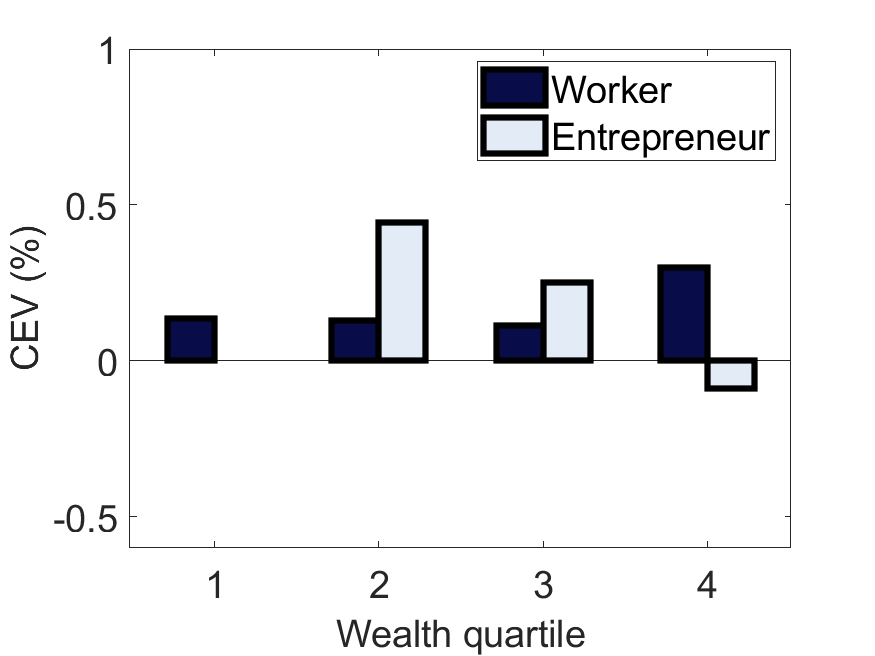
\includegraphics[width=\textwidth]{\FigDir/comptran_CF2_cev_qo}
	\caption{CEV by wealth decile and occupation, no avoidance}
\end{subfigure} 
	\caption{}
	\label{fig:comptran_CEV}
	\floatfoot{\textit{Notes:} The welfare maximizing top marginal tax rate $\tau_h$ is 0.464 in the benchmark economy and 0.480 in the counterfactual economy.}
\end{figure}	


\bibliographystyle{aer}
\bibliography{DKST_biblio2}
	
\end{document}
